\chapter{Tree decomposition}

Firstly we may recall that: $K_{5} \nleq_{m} G$ iff $G$ is obtained from planar graphs and $W_{8}$'s by clique-sums. When we draw the graphs expanding by the clique sums we may notice a somewhat tree structure that they generate. Now we will define it and see it properly.

\section{Basics}

\begin{defn}
	A \textbf{tree decomposition} $(T, \beta)$ of graph $G$ is when $T$ is a tree and $\beta: V(T) \to 2^{V(G)}$ (\textit{called bags}) such that
	
	\begin{enumerate}[(1)]
		\item $(\forall uv \in E(G)) (\exists x \in V(T)): u,v \in \beta(x)$ or by words every edge is contained in a bag.
		\item $\forall v \in V(G)$ the set $\{x \in V(T) : v \in \beta(x)\}$ induces a non-empty connected subtree of $T$.
	\end{enumerate}
\end{defn}

\begin{lemma}
	If $(T, \beta)$ is a tree decomposition of $G$, $K \subseteq V(G)$ is a clique in $G$ then $(\exists x \in V(T)) : K \subseteq \beta(x)$.
\end{lemma}

\begin{proof}
	For contradiction suppose it is not true. Thus $(\forall x \in V(T)) (\exists v_{x} \in K) : v_{x} \notin \beta(x)$. We define "arrows" for each vertex which points to the set $\{y : v_{x}' \notin \beta(x)\}$. Thus there is $|V(T)|$ of "arrows" but because it is a tree there is $|E(T)| = |V(T)| - 1 < |V(T)|$. So at least one edge must have two "arrows". Therefore there is no $y \in V(T)$ with $v_{x}, v_{x'} \in \beta(x)$ so $K$ clique implies that $v_{x}$ and $v_{x'}$ are adjacent. This is contradiction with (1) from definition.
\end{proof}

\section{Torso}

\begin{defn}
	$(T, \beta)$ is tree decomposition of $G$ and let $x \in V(T)$ then the \textbf{torso} of $x$. is $G[\beta(x)] + $ cliques on $\beta(x) \cap \beta(y)$ for every $xy \in E(T)$.
\end{defn}

This definition may not be clear to everybody so lets take a look at an example. On picture \ref{example-torso} we may see the original graph \ref{g-torso} and on picture \ref{t-torso} we may see the tree decomposition. Now we set $x$ to be \texttt{\textcolor{mygreen}{B}\textcolor{myorange}{G}\textcolor{myblue}{E}}. Now for the torso itself we create a three vertices \texttt{B}, \texttt{G} and \texttt{E} where there is no induced edge. Then for the neighbors \texttt{ABG} we add a edge between \texttt{B} and \texttt{G}. For \texttt{BED} we add an edge between \texttt{B} and \texttt{E} and lastly for \texttt{EGF} we add \texttt{E}--\texttt{G} edge. And finally we get what is drawn on picture \ref{torso}.

\begin{figure}[!ht]\centering
	\begin{subfigure}{0.3\textwidth}\centering
		\begin{tikzpicture}[node distance={14mm}, thick, main/.style = {draw, circle}]
			\node[main] (1) {A};
			\node[main] (2) [below right of=1, color = mygreen] {B};
			\node[main] (3) [above right of=2] {C};
			\node[main] (4) [below right of=3] {D};
			\node[main] (5) [below of=4, color = myblue] {E};
			\node[main] (6) [below left of=5] {F};
			\node[main] (7) [left of=6, color = myorange] {G};
			\node[main] (8) [above left of=7] {H};
			\path
				(1) edge (2)
				(2) edge (3)
				(3) edge (4)
				(4) edge (5)
				(5) edge (6)
				(6) edge (7)
				(7) edge (8)
				(8) edge (1);
		\end{tikzpicture}
		\caption{Original graph $G$.}
		\label{g-torso}
	\end{subfigure}
	\begin{subfigure}{0.35\textwidth}\centering
		\begin{tikzpicture}[node distance={14mm}, thick, main/.style = {draw, circle}]
			\node[main] (1) {\tiny{A\textcolor{myorange}{G}H}};
			\node[main] (2) [below right of=1] {{\tiny A\textcolor{mygreen}{B}\textcolor{myorange}{G}}};
			\node[main] (3) [below right of=2] {{\tiny \textcolor{mygreen}{B}\textcolor{myorange}{G}\textcolor{myblue}{E}}};
			\node[main] (4) [above right of=3] {{\tiny \textcolor{mygreen}{B}\textcolor{myblue}{E}D}};
			\node[main] (5) [above right of=4] {{\tiny \textcolor{mygreen}{B}CD}};
			\node[main] (6) [below of=3] {{\tiny \textcolor{myblue}{E}\textcolor{myorange}{G}F}};
			\path
			(1) edge (2)
			(2) edge (3)
			(3) edge (4)
			(4) edge (5)
			(3) edge (6);
		\end{tikzpicture}
		\caption{Tree decomposition of $G$.}
		\label{t-torso}
	\end{subfigure}
	\begin{subfigure}{0.3\textwidth}\centering
		\begin{tikzpicture}[node distance={14mm}, thick, main/.style = {draw, circle}]
			\node[main] (1) {\textcolor{mygreen}{B}};
			\node[main] (2) [below right of=1] {\textcolor{myblue}{E}};
			\node[main] (3) [below left of=1] {\textcolor{myorange}{G}};
			\path
			(1) edge (2)
			(2) edge (3)
			(3) edge (1);
		\end{tikzpicture}
		\caption{Actual \textbf{torso} of $x$.}
		\label{torso}
	\end{subfigure}
	\caption{An example of \textbf{torso.}}
	\label{example-torso}
\end{figure}

\begin{lemma}
	Let $\mathcal{G}$ be a class of graphs. $G$ is obtained by clique-sums from graphs belonging to $\mathcal{G}$ iff $G$ has a tree decomposition whose torsos belongs to $\mathcal{G}$.
\end{lemma}

\begin{proof}
	Firstly the "$\Leftarrow$" is easy since when taken the tree decomposition torso we may see that it is somewhat the same as clique-sum of the graphs.
	
	Next we have "$\Rightarrow$" for them we will prove it by induction on the number of terms.
	
	\begin{enumerate}[(i)]
		\item When we have one term than the whole $G \in \mathcal{G}$ and we take a tree decomposition with only one vertex having all vertices from $G$.
		\item Now we have $G = G_{1} \bigoplus_{K} G_{2}$ thus there by induction hypothesis we have $(T_{1}, \beta_{1})$ and $(T_{2}, \beta_{2})$ tree decompositions of their respected graphs $G_{1}$ and $G_{2}$. By lemma there exists a bag with clique $K$ in both $T_{1}$ and $T_{2}$. So we create $T$ by adding edge between those bags in $T_{1}$ and $T_{2}$. So $(T, \beta = \beta_{1} \cup \beta_{2})$ will be the tree decomposition. While it may seem easy it is necessary to show that all properties holds. Every edge is contained in at least one bag since we did not added no edge. Secondly all $x$ induces a non-empty connected subtree.
		
		Also we have to take a look at the torsos we are getting from this tree decomposition. For those bags not having new edge it is still the same as before and for bag $\beta(x)$ which $K \subseteq \beta(x)$ we see that its only intersection is $K$ so it won't change any torso because it is a clique.
	\end{enumerate}
\end{proof}

\section{Tree width}

So we introduced basic tree decomposition but now we take a deeper look at some special cases of them.

\begin{defn}
	\textbf{Width} of $(T, \beta)$ is $\max_{x \in V(T)} (|\beta(x)|) -1$.
\end{defn}

\begin{defn}
	We denote $\text{tw}(G) = \min$ width of $(T, \beta)$ for all $(T, \beta)$ tree decompositions of $G$. It is called the \textbf{treewidth}.
\end{defn}

We may recall and extend that for $k \leq 4$: $K_{k} \nleq_{m} G$ iff $G$ is obtained by clique-sum from graphs with $\leq k-1$ vertices iff $G$ having tree decomposition $(T, \beta)$ such that $(\forall x \in V(T)) : |\beta(x)| \leq k-1$ which means that $\text{width}(T, \beta) \leq k - 2$ iff $\text{tw}(G) \leq k - 2$.

We would now need $\{G : \text{tw}(G) \leq k\}$ is minor-closed.

\begin{observ}
	$H \leq_{m} G \Rightarrow \text{tw}(H) \leq \text{tw}(G)$
\end{observ}

\begin{proof}
	We may see all possible operations. First deletion of vertex may only decrease the value. Second the deletion of edge may also only decrease the value. Lastly for contracting an edge $uv$ we overwrite all these vertices to $w$ and change the edges. This is easily seen that it will only decrease the value or it will stay the same.
\end{proof}

From that we get that $\exists \mathcal{F}_{k}$ $\text{tw}(G) \leq k$ iff $(\forall F \in \mathcal{F}_{k}) F \nleq_{m} G$. Also for some simple values we know $\mathcal{F}_{1} = \{K_{3}\}$ also $\mathcal{F}_{2} = \{K_{4}\}$ and for $\mathcal{F}_{3} = \{K_{5, \dots }\}$ where it is known but not that important.

\section{Bramble}

\begin{defn}
	Bramble $\mathcal{B} \subseteq 2^{V(G)}$ such that
	
	\begin{enumerate}[(1)]
		\item $(\forall B \in \mathcal{B}) B \neq \emptyset$ and $G[B]$ is connected.
		\item $(\forall B_{1}, B_{2} \in \mathcal{B})$ $G[B_{1} \cup B_{2}]$ is connected.
	\end{enumerate}
\end{defn}

As previously we will take a look at an example of a bramble so that a reader gets a better grasp on this definition. On the picture \ref{rumble-example} we may see a graph $G$ where there is Bramble $\mathcal{B} = \{B_{1}, B_{2}, B_{3}, B_{4}\}$.

\begin{figure}[!ht]\centering
	\begin{tikzpicture}[node distance={15mm}, thick, main/.style = {draw, thick, circle}]
		\node[main] (1) [color=black] {{\tiny $B_{3}$}};
		\node[main] (2) [right of=1] [color=purple] {{\tiny $B_{3}$, $B_{4}$}};
		\node[main] (3) [right of=2] [color=myorange] {{\tiny $B_{1}$}};
		\node[main] (4) [below of=1] [color=purple] {{\tiny $B_{3}$, $B_{4}$}};
		\node[main] (5) [right of=4] [color=purple] {{\tiny $B_{4}$}};
		\node[main] (6) [right of=5] [color=myorange] {{\tiny $B_{1}$}};
		\node[main] (7) [below of=4] [color=blue] {{\tiny $B_{2}$}};
		\node[main] (8) [right of=7] [color=blue] {{\tiny $B_{2}$}};
		\node[main] (9) [right of=8] [color=myorange] {{\tiny $B_{1}$}};
		\path
			(1) edge (2) (2) edge (5)
			(2) edge (3) (3) edge (6)
			(1) edge (4) (5) edge (8)
			(4) edge (7) (6) edge (9)
			(4) edge (5) (5) edge (6)
			(7) edge (8) (8) edge (9);
	\end{tikzpicture}
	\caption{Bramble of a graph $G$.}
	\label{rumble-example}
\end{figure}

\begin{defn}
	Set $X$ \textbf{hits} the Bramble $\mathcal{B}$ if $(\forall B \in \mathcal{B}) B \cap X \neq \emptyset$.
\end{defn}

For the previous example a hit could be all these vertices highlighted on the picture \ref{hit}.

\begin{figure}[!ht]\centering
	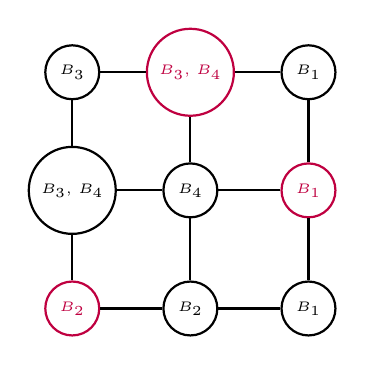
\begin{tikzpicture}[node distance={15mm}, thick, main/.style = {draw, thick, circle}]
		\node[main] (1) {{\tiny $B_{3}$}};
		\node[main] (2) [right of=1] [color=purple] {{\tiny $B_{3}$, $B_{4}$}};
		\node[main] (3) [right of=2] {{\tiny $B_{1}$}};
		\node[main] (4) [below of=1] {{\tiny $B_{3}$, $B_{4}$}};
		\node[main] (5) [right of=4] {{\tiny $B_{4}$}};
		\node[main] (6) [right of=5] [color=purple] {{\tiny $B_{1}$}};
		\node[main] (7) [below of=4] [color=purple] {{\tiny $B_{2}$}};
		\node[main] (8) [right of=7] {{\tiny $B_{2}$}};
		\node[main] (9) [right of=8] {{\tiny $B_{1}$}};
		\path
			(1) edge (2) (2) edge (5)
			(2) edge (3) (3) edge (6)
			(1) edge (4) (5) edge (8)
			(4) edge (7) (6) edge (9)
			(4) edge (5) (5) edge (6)
			(7) edge (8) (8) edge (9);
	\end{tikzpicture}
	\caption{Brumble of a graph $G$.}
	\label{hit}
\end{figure}

\begin{lemma}[duality]
	If $(T, \beta)$ is a tree decomposition of $G$ and $\mathcal{B}$ is a bramble then $(\exists x \in V(T)) \beta(x)$ hits the bramble.
\end{lemma}

\begin{observ}
	If $(T, \beta)$ is a tree decomposition of $G$ and $F \subseteq G$ connected, then $\{x \in V(T) : \beta(x) \cap V(F) \neq \emptyset\}$ induces a connected subtree of $T$.
\end{observ}

\begin{proof}
	By induction on $|V(F)|$.
	
	\begin{enumerate}[(i)]
		\item $|V(F)| = 1$ is by the definition.
		\item $|V(F)| > 1$ consider $v \in V(F)$ such that $F - v$ is connected (we could take a leaf from a spanning tree of $F$) so we use an induction hypothesis $F - v$. We take a subtree on $V(F-b)$ and $\{v\}$. By the definition $\exists y: u,v \in \beta(y)$.
	\end{enumerate}
\end{proof}

\begin{proof}[Proof of lemma]
	For contradiction suppose it is false. So $(\forall x \in V(T)) \beta (x)$ does not hit $\mathcal{B}$ so we have $B_{x} \in \mathcal{B}$ disjoint from $\beta(x)$. By lemma $B_{x}$ forms in $(T, \beta)$ a connected subtree. Again we assign "arrows" to vertices pointing to $x$--$B_{x}$. Also there are more arrows than edges so at least one edge has two "arrows". We can find $B_{x}$ and $B_{x'}$ not in the same bag so they are disjoint. This is a contradiction by the definition.
\end{proof}

Note that on $K$ clique the bramble is $\mathcal{B} = \{\{u\}: u \in K\}$.

\begin{defn}
	\textbf{Order} of bramble is defined as $\text{order}(\mathcal{B}) = \min (|X|): X \text{ hits } \mathcal{B}$.
\end{defn} 

\begin{cor}
	$\text{tw}(G) \geq \max (\text{order}(\mathcal{B})) - 1$ for all $\mathcal{B}$ rumble in $G$.
\end{cor}

\begin{rem}
	It can be proven so that there is equality not inequality. But we will not be showing this result since it is not so easy.
\end{rem}

In other words we may rewrite the previous findings as a similiar lemma.

\begin{lemma}
	$\forall$ tree decompositions $(T, \beta)$ and $\forall$ bramble $\mathcal{B}$ in $G$ it holds that
	
	$$
	\text{width}(T, \beta) \geq \text{order}(\mathcal{B}) - 1
	$$
\end{lemma}

\subsection{$n \times n$ grid}

Now we will take a look at a simple example of a graph and its tree decomposition and bramble. This graph is an $n \times n$ grid where every neighbor is connected, one can be seen on picture \ref{nbynmatrix}.

\begin{figure}[!ht]\centering
	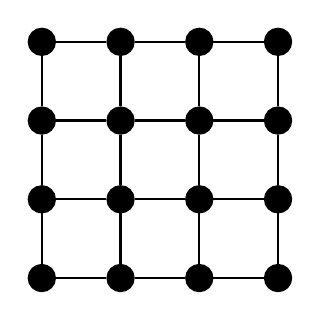
\begin{tikzpicture}[node distance={10mm}, thick, main/.style = {draw, circle, fill}]
		\node[main] (1) {};
		\node[main] (2) [right of=1] {};
		\node[main] (3) [right of=2] {};
		\node[main] (4) [below of=1] {};
		\node[main] (5) [right of=4] {};
		\node[main] (6) [right of=5] []{};
		\node[main] (7) [below of=4] []{};
		\node[main] (8) [right of=7] {};
		\node[main] (9) [right of=8] {};
		\node[main] (10) [below of=7] {};
		\node[main] (11) [right of=10] {};
		\node[main] (12) [right of=11] {};
		\node[main] (13) [right of=3] {};
		\node[main] (14) [right of=6] {};
		\node[main] (15) [right of=9] {};
		\node[main] (16) [right of=12] {};
		\path
			(1) edge (2) (2) edge (5) (14) edge (13)
			(2) edge (3) (3) edge (6) (14) edge (15)
			(1) edge (4) (5) edge (8) (15) edge (16)
			(4) edge (7) (6) edge (9) (7) edge (10)
			(4) edge (5) (5) edge (6) (8) edge (11)
			(7) edge (8) (8) edge (9) (9) edge (12)
			(10) edge (11) (11) edge (12)
			(12) edge (16) (9) edge (15)
			(6) edge (14) (3) edge (13);
	\end{tikzpicture}
	\caption{$n \times n$ matrix example.}
	\label{nbynmatrix}
\end{figure}

When we examine a tree decomposition we may easily find one such with tree width $2n$. That is we take 2 rows that are adjacent. But much better tree decomposition is when we take it like it is visualized on picture \ref{treewidthnbyn}. This gives us a tree decomposition with width $n+1$.

\begin{figure}[!ht]\centering
	\begin{subfigure}{0.25\textwidth}
		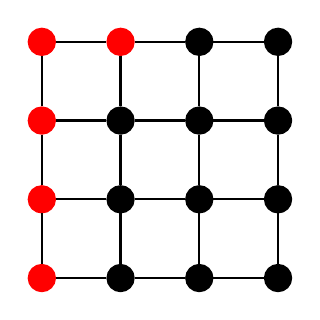
\begin{tikzpicture}[node distance={10mm}, thick, main/.style = {draw, circle, fill}]
			\node[main] (1) [color = red] {};
			\node[main] (2) [right of=1] [color = red] {};
			\node[main] (3) [right of=2] {};
			\node[main] (4) [below of=1] [color = red] {};
			\node[main] (5) [right of=4] {};
			\node[main] (6) [right of=5] {};
			\node[main] (7) [below of=4] [color = red] {};
			\node[main] (8) [right of=7] {};
			\node[main] (9) [right of=8] {};
			\node[main] (10) [below of=7] [color = red] {};
			\node[main] (11) [right of=10] {};
			\node[main] (12) [right of=11] {};
			\node[main] (13) [right of=3] {};
			\node[main] (14) [right of=6] {};
			\node[main] (15) [right of=9] {};
			\node[main] (16) [right of=12] {};
			\path
			(1) edge (2) (2) edge (5) (14) edge (13)
			(2) edge (3) (3) edge (6) (14) edge (15)
			(1) edge (4) (5) edge (8) (15) edge (16)
			(4) edge (7) (6) edge (9) (7) edge (10)
			(4) edge (5) (5) edge (6) (8) edge (11)
			(7) edge (8) (8) edge (9) (9) edge (12)
			(10) edge (11) (11) edge (12)
			(12) edge (16) (9) edge (15)
			(6) edge (14) (3) edge (13);
		\end{tikzpicture}
	\end{subfigure}
	\begin{subfigure}{0.25\textwidth}
		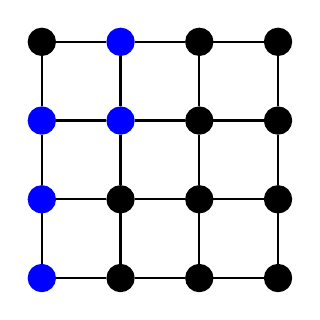
\begin{tikzpicture}[node distance={10mm}, thick, main/.style = {draw, circle, fill}]
			\node[main] (1) {};
			\node[main] (2) [right of=1] [color = blue] {};
			\node[main] (3) [right of=2] {};
			\node[main] (4) [below of=1] [color = blue] {};
			\node[main] (5) [right of=4] [color = blue] {};
			\node[main] (6) [right of=5] {};
			\node[main] (7) [below of=4] [color = blue] {};
			\node[main] (8) [right of=7] {};
			\node[main] (9) [right of=8] {};
			\node[main] (10) [below of=7] [color = blue] {};
			\node[main] (11) [right of=10] {};
			\node[main] (12) [right of=11] {};
			\node[main] (13) [right of=3] {};
			\node[main] (14) [right of=6] {};
			\node[main] (15) [right of=9] {};
			\node[main] (16) [right of=12] {};
			\path
			(1) edge (2) (2) edge (5) (14) edge (13)
			(2) edge (3) (3) edge (6) (14) edge (15)
			(1) edge (4) (5) edge (8) (15) edge (16)
			(4) edge (7) (6) edge (9) (7) edge (10)
			(4) edge (5) (5) edge (6) (8) edge (11)
			(7) edge (8) (8) edge (9) (9) edge (12)
			(10) edge (11) (11) edge (12)
			(12) edge (16) (9) edge (15)
			(6) edge (14) (3) edge (13);
		\end{tikzpicture}
	\end{subfigure}
	\begin{subfigure}{0.25\textwidth}
		\begin{tikzpicture}[node distance={10mm}, thick, main/.style = {draw, circle, fill}]
			\node[main] (1) {};
			\node[main] (2) [right of=1] [color = myorange] {};
			\node[main] (3) [right of=2] {};
			\node[main] (4) [below of=1] {};
			\node[main] (5) [right of=4] [color = myorange] {};
			\node[main] (6) [right of=5] {};
			\node[main] (7) [below of=4] [color = myorange] {};
			\node[main] (8) [right of=7] [color = myorange] {};
			\node[main] (9) [right of=8] {};
			\node[main] (10) [below of=7] [color = myorange] {};
			\node[main] (11) [right of=10] {};
			\node[main] (12) [right of=11] {};
			\node[main] (13) [right of=3] {};
			\node[main] (14) [right of=6] {};
			\node[main] (15) [right of=9] {};
			\node[main] (16) [right of=12] {};
			\path
			(1) edge (2) (2) edge (5) (14) edge (13)
			(2) edge (3) (3) edge (6) (14) edge (15)
			(1) edge (4) (5) edge (8) (15) edge (16)
			(4) edge (7) (6) edge (9) (7) edge (10)
			(4) edge (5) (5) edge (6) (8) edge (11)
			(7) edge (8) (8) edge (9) (9) edge (12)
			(10) edge (11) (11) edge (12)
			(12) edge (16) (9) edge (15)
			(6) edge (14) (3) edge (13);
		\end{tikzpicture}
	\end{subfigure}
	\caption{First three bags of tree decomposition.}
	\label{treewidthnbyn}
\end{figure}

So we can say that $\text{tw}(n \times n \text{grid}) \leq n$. Can we construct some with even lower width? We can use the previous lemma and construct a bramble which can be seen on picture \ref{bramblenbyn}. So there are two special sets on the sides and then we have all the crosses in the rest of the grid. This will lead to bramble $\mathcal{B}$ of order $\geq n+1$. We must select two points for two special sets and points on the diagonal for example. Therefore with the use of the lemma we also have that $\text{tw}(n \times n \text{grid}) \geq n$ thus it has to be equal.

\begin{figure}[!ht]\centering
	\begin{tikzpicture}[node distance={10mm}, thick, main/.style = {draw, circle, fill}]
		\node[main] (1) {};
		\node[main] (2) [right of=1] [color = purple] {};
		\node[main] (3) [right of=2] {};
		\node[main] (4) [below of=1] [color = purple] {};
		\node[main] (5) [right of=4] [color = purple] {};
		\node[main] (6) [right of=5] [color = purple] {};
		\node[main] (7) [below of=4] {};
		\node[main] (8) [right of=7] [color = purple] {};
		\node[main] (9) [right of=8] {};
		\node[main] (10) [below of=7] [color = blue] {};
		\node[main] (11) [right of=10] [color = blue] {};
		\node[main] (12) [right of=11] [color = blue] {};
		\node[main] (13) [right of=3] [color = myorange] {};
		\node[main] (14) [right of=6] [color = myorange] {};
		\node[main] (15) [right of=9] [color = myorange] {};
		\node[main] (16) [right of=12] [color = myorange] {};
		\path
		(1) edge (2) (2) edge (5) (14) edge (13)
		(2) edge (3) (3) edge (6) (14) edge (15)
		(1) edge (4) (5) edge (8) (15) edge (16)
		(4) edge (7) (6) edge (9) (7) edge (10)
		(4) edge (5) (5) edge (6) (8) edge (11)
		(7) edge (8) (8) edge (9) (9) edge (12)
		(10) edge (11) (11) edge (12)
		(12) edge (16) (9) edge (15)
		(6) edge (14) (3) edge (13);
	\end{tikzpicture}
	\caption{A bramble for $n \times n$ grid.}
	\label{bramblenbyn}
\end{figure}

With that we can state that if $n \times n$ grid $\leq_{m} G$ then $\text{tw}(G) \geq n$. Which also means that we can construct planar graph with any given tree width.

\begin{thm}
	$\text{tw}(G) \geq \Omega(n^{10})$ then $n \times n$ grid $\leq_{m} G$.
\end{thm}

This is quite recent discovery and long time it was only exponential. Now it is polynomial. We won't be proving this but instead we take a look at something in a way similiar.

\subsection{$n$-ladder}

$n$-ladder is graph that looks like a $2 \times n$ grid. Or just like it is on the picture \ref{nladder}.

\begin{figure}[!ht]\centering
	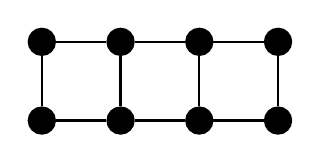
\begin{tikzpicture}[node distance={10mm}, thick, main/.style = {draw, circle, fill}]
		\node[main] (1) {};
		\node[main] (2) [right of=1] {};
		\node[main] (3) [right of=2] {};
		\node[main] (4) [below of=1] {};
		\node[main] (5) [right of=4] {};
		\node[main] (6) [right of=5] {};
		\node[main] (13) [right of=3] {};
		\node[main] (14) [right of=6] {};
		\path
		(1) edge (2) (2) edge (5)
		(2) edge (3) (3) edge (6)
		(1) edge (4) (13) edge (14)
		(4) edge (5) (5) edge (6)
		(6) edge (14) (3) edge (13);
	\end{tikzpicture}
	\caption{Example of an $n$-ladder.}
	\label{nladder}
\end{figure}

\begin{thm}
	$\text{tw}(G) \geq 2n^{2} - 1 \Rightarrow$ $n$-ladder $\leq_{m} G$.
\end{thm}

We won't be proving this straightforward. Instead we will prove something similiar which implies this theorem.

\begin{thm}
	If $G$ contains a bramble $\mathcal{B}$ of order $\geq 2n^2$ then $n$-ladder $\leq_{m} G$.
\end{thm}

Firstly we will show some lemmas.

\begin{lemma}
	If $\mathcal{B}$ is a bramble in $G$, then there exists path $P \subseteq G$ such that
	
	$$
	\forall B \in \mathcal{B} : B \cap V(P) \neq \emptyset
	$$
\end{lemma}

\begin{proof}
	Lets take $B_{1} \in \mathcal{B}$ and $x \in V(G)$ such that $x \in B_{1}$. If it is contained in all sets from bramble then we are done. Otherwise find such $B_{2} \in \mathcal{B}$ that does not contain it. Then by the bramble properties we are able to find path from $x$ to $B_{2}$. If now the path is contained in all sets from bramble we are done. Otherwise we iterate.
\end{proof}

\begin{lemma}
	Suppose $\mathcal{B}$ is a bramble, $\mathcal{B} = \mathcal{B}_{1} \dot \cup \mathcal{B}_{2}$. Then $\mathcal{B}_{1}$ and $\mathcal{B}_{2}$ are also brambles and
	
	$$
	\text{order}(\mathcal{B}) \leq \text{order}(\mathcal{B}_{1}) + \text{order}(\mathcal{B}_{2})
	$$
\end{lemma}

\begin{proof}
	This is straightforward from the definition of the bramble and some observations.
\end{proof}

\begin{proof}[Proof of theorem]
	Let $P$ be a path intersecting all sets in $\mathcal{B}$. let $P_{1}$ be a path segment.
	
	$$
	\mathcal{B}_{1} = \{B \in \mathcal{B} : B \cap V(P_{1}) \neq \emptyset\}
	$$
	
	Choose $P_{1}$ shortest such that $\text{order}(\mathcal{B}_{1}) \geq n^2$. We also claim there need to be equality since we are looking for the shortest path. Now let $\mathcal{B}_{2} = \mathcal{B} \setminus \mathcal{B}_{1}$. By the lemma we know $\text{order}(\mathcal{B}_{2}) \geq n^{2}$. Also we set $P_{2}$ to path intersecting all sets in $\mathcal{B}_{2}$.
	
	The claim is that $G$ contains $n^{2}$ disjoint paths from $P_{1}$ to $P_{2}$, By Merger's theorem if there is cut of such size there must as many disjoint paths. If we would remove $< n^{2}$ vertices there would exists in both paths such $B_{1}$ and $B_{2}$ respectively so the are not hit. By their properties they induce a connected subgraph. So there is a path. This proves the claim.
	
	We also remind ourselves a theorem
	
	\begin{thm}[Erdos-Szekeres]
		Every sequence of length $n^2$ contains a monotone sub-sequence of length $n$.
	\end{thm}
	
	Thus if the sub-sequence is increasing we just find $n$ paths thus an $n$-ladder. If it is decreasing we just flip one path and find the same result.
\end{proof}

Now we will see an application of this theorem.

\begin{thm}[Erdos-Prosa]
	There exists $f$ such that $\forall k$ $\forall G$ either
	
	\begin{itemize}
		\item $G$ contains more than $k$ pairwise distinct cycles or
		\item $\exists X \subseteq V(G)$, $|X| \leq f(X)$ such that $G - X$ does not contain cycle.
	\end{itemize}
\end{thm}

They proved it for $f(k) = O(k \log k)$, but we will show for other $f$ that exploits our previous theorem.

\begin{defn}
	$n_{1}, n_{2}, \dots, n_{m} \in \N$ is \textbf{$k$-bounded} if $n_{1}, n_{2}, \dots, n_{m} \leq k/2$ and $\sum_{i} n_{i} \leq k$.
\end{defn}

Now we set our $f$ to be: $f(0) =0$ and

$$
f(k) = 2(2k+2)^2 + \max_{I \ k-\text{bounded}} \sum_{i \in I} f(i).
$$

\begin{proof}
	Suppose $G$ contains $\leq k$ disjoint cycles. We will be proving this by induction on $k$.
	
	$$
	\mathcal{B} = \{B \subseteq V(G) : G[B] \text{ is connected, contains } > k/2 \text{ disjoint cycles}\}
	$$
	
	is a bramble. Any two $B_{1}$ and $B_{2}$ must intersect otherwise we have a contradiction with our assumption of not having $k$ cycles. If $\text{order}(\mathcal{B}) \geq 2(2k+2)^2$ then there is $2k+2$-ladder as a minor of $G$. This means there would be $k+1$ pairwise distinct cycles which is a contradiction.
	
	So $(\exists X : |X| < 2(2k+2)^2) X \text{ hits } \mathcal{B}$. Now take $G - X$ and denote their components as $K_{1}, K_{2}, \dots$. let $n_{i}$ be the number of pairwise distinct cycles in $K_{i}$. We may see that the sum $\sum n_{i} \leq k$ otherwise it is a contradiction with the assumption. And also $n_{i} \leq k/2$ for any $i$. Due to the bramble properties. Thus this sequence is $k$-bounded. Apply induction on components. We get $|X_{i}| \leq f(n_{i})$ by induction hypothesis. Thus
	
	$$
	G = (X \cup \bigcup_{i} X_{i}) \text{ is a forest and}
	$$
	
	$$
	|G - (X \cup \bigcup_{i} X_{i})| \leq f(k)
	$$
\end{proof}